% main.tex

\documentclass[12pt, a4paper]{article}

% Preamble dosyasını çağır
% preamble.tex

% Türkçe karakter desteği ve dil ayarları
\usepackage[utf8]{inputenc}
\usepackage[T1]{fontenc}
\usepackage[turkish]{babel}
% babel Türkçe'de eşittir işaretinin shorthand olmasını sevmiyor gibi
\AtBeginDocument{\shorthandoff{=}}

% Satır aralığı: 1.5 (Türkpatent zorunluluğu)
\usepackage{setspace}
\onehalfspacing

% Metin sayfaları için sayfa kenar boşlukları (Üst 2-4 cm, Sol 2.5-4 cm, Sağ 2-3 cm, Alt 2 cm)
\usepackage[top=3cm, left=3cm, right=2.5cm, bottom=2cm]{geometry}

% Satır numaralandırması (Her 5 satırda bir)
\usepackage[left]{lineno}
\modulolinenumbers[4]

% Sayfa numaralandırması (Alt orta kısımda)
\usepackage{fancyhdr}
\pagestyle{fancy}
\fancyhf{} % Üst ve alt bilgileri temizle
\renewcommand{\headrulewidth}{0pt} % Üst çizgi kalınlığını sıfırla
\cfoot{\thepage} % Sayfa numarasını alta ortala 

% Resim ekleme desteği ve resimlerin aranacağı klasör
\usepackage{graphicx}
\graphicspath{{sekiller/}}

% Resim sayfaları (04-resimler.tex) için özel kenar boşluğu ve sayfa numaralandırması
% ayarlarını ana belgede veya ilgili dosyanın içinde yöneteceğiz.


\begin{document}

% Metin kısımları için satır numaralarını aktif et
\linenumbers

% Bölümleri sırasıyla dahil et (Her \include komutu yeni bir sayfadan başlar)
% 01-tarifname.tex

\begin{center}
    \textbf{TARİFNAME} \\
    \vspace{1em}
    \textbf{BULUŞUN BAŞLIĞINI BURAYA YAZINIZ}
\end{center}

\section*{Teknik Alan}
% Buluşun hangi teknik alanla ilgili olduğu bu kısımda kısaca belirtilir.
Bu buluş, ... ile ilgilidir.

\section*{Önceki Teknik}
% Buluşun anlaşılması için yurt içi ve yurt dışındaki benzer buluş, teknoloji ya da ürünler burada anlatılır.

\section*{Buluşun Amacı}
% Buluşun tekniğin bilinen durumuna kıyasla getirdiği yenilikler ve çözdüğü problemler anlatılmalıdır.

\section*{Şekillerin Açıklaması}
% Başvuruda resim bulunuyorsa, bu resimlerdeki şekillerin kısa açıklamaları liste halinde verilir.
% Örnek: Şekil 1: Buluş konusu ...'nın perspektif görünüşüdür.

\section*{Şekillerdeki Referansların Açıklaması}
% Şekillerde bulunan parçalar vb. referans işaretleri ile gösterilir.
% Örnek:
% 1: Gövde
% 2: Kapak

\section*{Buluşun Açıklaması}
% Buluşun tüm detayı ile anlatıldığı kısımdır.

\section*{Buluşun Sanayiye Uygulanma Biçimi}
% Buluşun nerede kullanılabileceği ve sanayiye nasıl uygulanacağı belirtilir.

% 02-istemler.tex

\begin{center}
    \textbf{İSTEMLER}
\end{center}

\begin{enumerate}
    \item Buluş, ... olup özelliği; ... içermesidir.
    
    \item İstem 1'e göre ... olup özelliği; ... olmasıdır.
\end{enumerate}

% 03-ozet.tex

\begin{center}
    \textbf{ÖZET} \\
    \vspace{1em}
    \textbf{BULUŞUN BAŞLIĞINI BURAYA YAZINIZ}
\end{center}

% Buluşla ilgili genel teknik bilgi verilen kısımdır. 
% Koruma kapsamının belirlenmesinde kullanılamaz.


% Resimler bölümünde satır numarası olmamalıdır
\nolinenumbers
% 04-resimler.tex

% Resim sayfaları için özel kenar boşlukları ayarlanır
\newgeometry{top=2.5cm, left=2.5cm, right=1.5cm, bottom=1cm}

% Resim sayfalarında sayfa numaralandırması "Mevcut Sayfa / Toplam Sayfa" şeklinde olmalıdır
\fancyhf{} 
\renewcommand{\headrulewidth}{0pt}
\cfoot{\thepage \ / \pageref{ResimlerSonSayfa}}

\begin{center}
    % ÖNEMLİ BİLGİ: 
    % Türkpatent kurallarına göre resimlerde (siyah dışında) renk ve gölgelendirme kullanılmaz. 
    % Şekillerin içi boyalı veya siyah dolu olmamalıdır (tarama çizgileri kullanılabilir).
    % Resimlerde antet veya sayfa çerçevesi bulunmamalıdır.
    
    % Şekil 1
    % Resim dosyalarınızı 'sekiller/' klasörüne yükleyip adını aşağıya yazınız.
    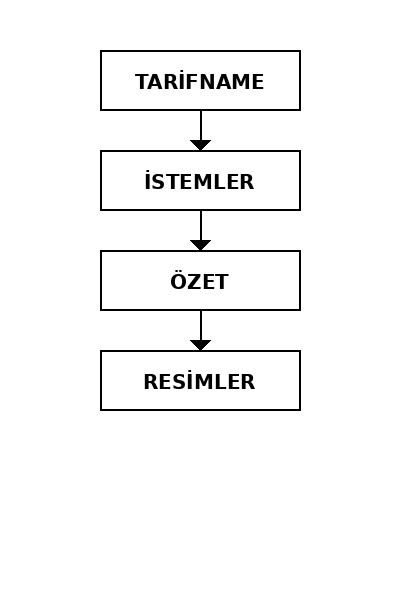
\includegraphics[width=0.8\textwidth]{sekil1} % Uzantı (.png, .jpg) yazmanıza gerek yoktur
    \vspace{2em}
    
    % Eğer aynı sayfaya birden fazla şekil ekleyecekseniz:
    % \includegraphics[width=0.8\textwidth]{sekil2}
    
\end{center}

% Yeni bir resim sayfasına geçmek için \newpage komutunu kullanabilirsiniz:
% \newpage
% \begin{center}
%     \includegraphics[width=0.8\textwidth]{sekil3}
% \end{center}

% Bu etiket, toplam resim sayfası sayısını hesaplamak için en sona eklenmiştir. Lütfen silmeyiniz.
\label{ResimlerSonSayfa}


\end{document}
